\documentclass[12pt]{beamer}

\usepackage{tikz}
\usetikzlibrary{automata}
\usetheme{EastLansing}

\title{GRAPH THEORY PRESENTATION }
\institute{Central Department of mathematics.}
\date{\today}
\begin{document}
\begin{frame}
\maketitle
\end{frame}
\begin{frame}[t]{Presenter Name list}
\begin{itemize}
  \item 1 Durga Pokharel
  \item 2.Kamala Lm Magar
  \item 3.Sadhna Limbu
  \item 4.Lekhak chand
  \item 5.Jaylal shah
  \item 6.Dinesh Khanel
  \item 7.Shefequr Rehman 
  \item 8.Krishna Chaudhary
\end{itemize}

\end{frame}
\begin{frame}[t]{contents}
\begin{enumerate}
\item Graph
\item Vertex
\item Arc
\item Directed graph
\item Undirected graph
\item Degree of digraph


 
\item weighted Graphs

\item Isomorphism,Cartesian product,Union
\item Walk,path,cycle,Girth


\end{enumerate}
 
\end{frame}
\begin{frame}[t]{Graph}
A graph is defined as G = (V,A).Where V is the set of vertices and A is the set of arcs.
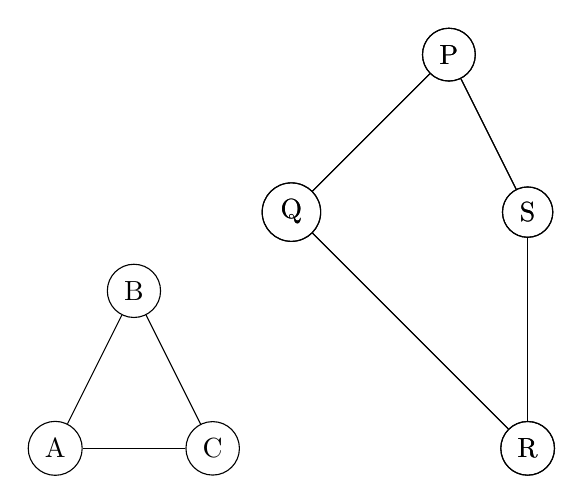
\begin{tikzpicture}
\node[circle ,draw=black](v1)at(5,5){P};
\node[circle,draw=black](v2) at (3,3){Q};
\node[circle,draw = black](v3) at(6,0) {R};
\node[circle,draw = black](v4) at(6,3){S};
\draw[-](v1)--(v2);
\draw[-](v2)--(v3);
\draw[-](v3)--(v4);
\draw[-](v4)--(v1);
\node[circle ,draw=black](v1)at(0,0){A};
\node[circle,draw=black](v2) at (1,2){B};
\node[circle,draw = black](v3) at(2,0) {C};

\draw[-](v1)--(v2);
\draw[-](v2)--(v3);
\draw[-](v3)--(v1);


\node[circle ,draw=black](v1)at(5,5){P};
\node[circle,draw=black](v2) at (3,3){Q};
\node[circle,draw = black](v3) at(6,0) {R};
\node[circle,draw = black](v4) at(6,3){S};
\draw[-](v1)--(v2);
\draw[-](v2)--(v3);
\draw[-](v3)--(v4);
\draw[-](v4)--(v1);
\end{tikzpicture}


\end{frame}
\begin{frame}[t]{vertex}
The set of vertices or node is denoted by V(D).\\.
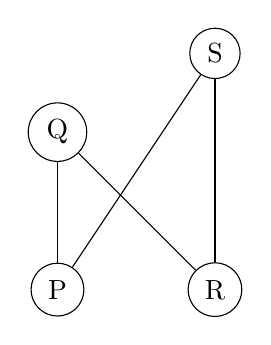
\begin{tikzpicture}
\node[circle ,draw=black](v1)at(0,0){P};
\node[circle,draw=black](v2) at (0,2){Q};
\node[circle,draw = black](v3) at(2,0) {R};
\node[circle,draw = black](v4) at(2,3){S};
\draw[-](v1)--(v2);
\draw[-](v2)--(v3);
\draw[-](v3)--(v4);
\draw[-](v4)--(v1);
\end{tikzpicture}\\
In above figure vertex are\\
 V = \{P,Q,R,S\}
\end{frame}
\begin{frame}[t]{Arcs}
The set of arcs are denoted by A(D).\\
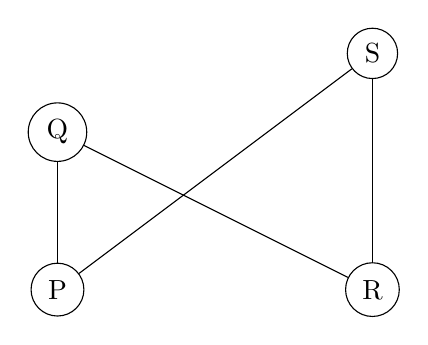
\begin{tikzpicture}
\node[circle ,draw=black](v1)at(0,0){P};
\node[circle,draw=black](v2) at (0,2){Q};
\node[circle,draw = black](v3) at(4,0) {R};
\node[circle,draw = black](v4) at(4,3){S};
\draw[-](v1)--(v2);
\draw[-](v2)--(v3);
\draw[-](v3)--(v4);
\draw[-](v4)--(v1);
\end{tikzpicture}\\
The arcs of above figure are\\
A = \{(P,Q),(P,S),(S,R),(R,S)\}\\
Note: In above figure we can take any node as incident node as well as end node.
\end{frame}
\begin{frame}[t]{Directed graph}
A graph is digraph if the arc(edge) are directed.\\
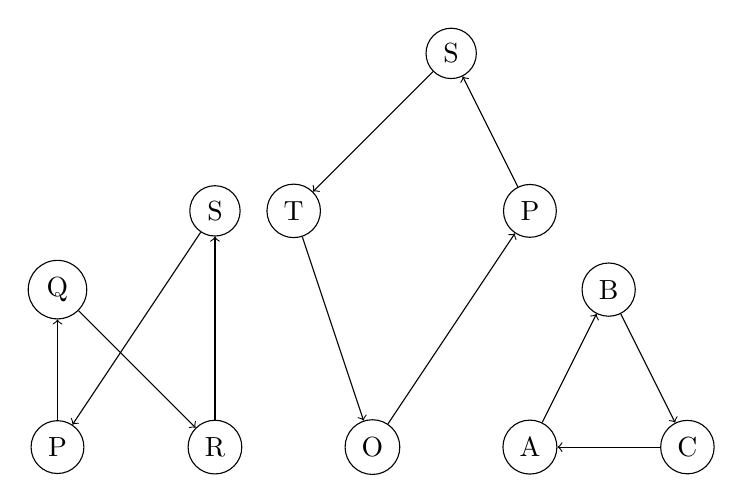
\begin{tikzpicture}
\node[circle ,draw=black](v1)at(0,0){P};
\node[circle,draw=black](v2) at (0,2){Q};
\node[circle,draw = black](v3) at(2,0) {R};
\node[circle,draw = black](v4) at(2,3){S};
\draw[->](v1)--(v2);
\draw[->](v2)--(v3);
\draw[->](v3)--(v4);
\draw[->](v4)--(v1);
\node[circle ,draw=black](v1)at(5,5){S};
\node[circle,draw=black](v2) at (3,3){T};
\node[circle,draw = black](v3) at(4,0) {O};
\node[circle,draw = black](v4) at(6,3){P};
\draw[->](v1)--(v2);
\draw[->](v2)--(v3);
\draw[->](v3)--(v4);
\draw[->](v4)--(v1);
\node[circle ,draw=black](v1)at(6,0){A};
\node[circle,draw=black](v2) at (7,2){B};
\node[circle,draw = black](v3) at(8,0) {C};

\draw[->](v1)--(v2);
\draw[->](v2)--(v3);
\draw[->](v3)--(v1);

\end{tikzpicture}

\end{frame}
\begin{frame}[t]{Undirected Graph}
If the arcs are not directed the graph is  undirected graph.\\
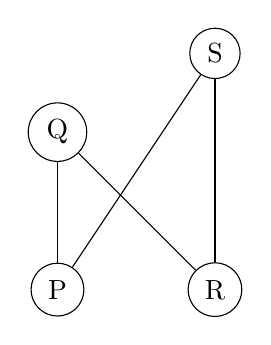
\begin{tikzpicture}
\node[circle ,draw=black](v1)at(0,0){P};
\node[circle,draw=black](v2) at (0,2){Q};
\node[circle,draw = black](v3) at(2,0) {R};
\node[circle,draw = black](v4) at(2,3){S};
\draw[-](v1)--(v2);
\draw[-](v2)--(v3);
\draw[-](v3)--(v4);
\draw[-](v4)--(v1);
\end{tikzpicture}\\
In above figure no arcs are directed from one vertex to another.
\end{frame}
\begin{frame}[t]{Types of Digraph}
\begin{itemize}
 \item Simple Digraph
 \item Parallel Digraph
 \item Multi Digraph
 \item Pseudo Digraph
\end{itemize}
1.Simple Digraph             

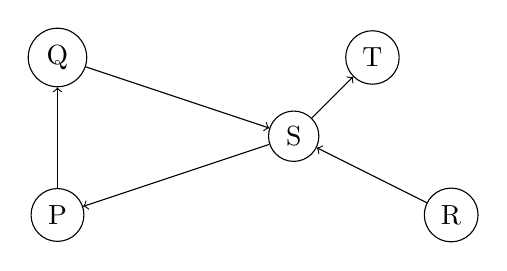
\begin{tikzpicture}
\node[circle ,draw=black](v1)at(0,0){P};
\node[circle,draw=black](v2) at (0,2){Q};
\node[circle,draw = black](v3) at(5,0){R};
\node[circle,draw = black](v4) at(3,1){S};
\node[circle,draw = black](v5) at (4,2){T};
\draw[->](v1)--(v2);
\draw[->](v2)--(v4);
\draw[->](v3)--(v4);
\draw[->](v4)--(v1);
\draw[->](v4)--(v5);
\end{tikzpicture}

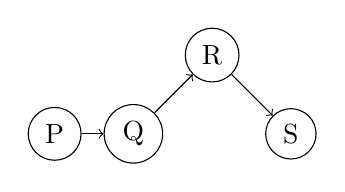
\begin{tikzpicture}
\node[circle ,draw=black](v1)at(4,1){P};
\node[circle,draw=black](v2) at (5,1){Q};
\node[circle,draw = black](v3) at(6,2) {R};
\node[circle,draw = black](v4) at(7,1){S};
\draw[->](v1)--(v2);
\draw[->](v2)--(v3);
\draw[->](v3)--(v4);


\end{tikzpicture}
\end{frame}
\begin{frame}[t]
2.Parallel
\begin{tikzpicture}
\node[circle ,draw=black](v1)at(4,1){a};
\node[circle,draw=black](v2) at (5,1){b};
\node[circle,draw = black](v3) at(6,2) {c};
\node[circle,draw = black](v4) at(7,1){d};
\node[circle,draw = black](v5) at (8,1){e};
\node[circle,draw = black](v6) at (9,0){f}
\draw[->](v1)--(v2);
\draw[->](v2)--(v3);
\draw[->](v3)--(v4);
\draw[->](v4)--(v5);
\draw[->](v5)--(v6);
\draw[->](v5)--(v6);
\end{tikzpicture}

\end{frame}
\end{document}